\newpage
\pagestyle{fancy}
\lhead{\textsc{Chapitre 1. Contexte général du projet}}
\renewcommand{\headrulewidth}{0.5pt}
\renewcommand{\footrulewidth}{0.5pt}
\chapter{Contexte général du projet}\setlength{\headheight}{28pt}
\label{ch1}
\minitoc
\newpage

\section{Introduction}
Ce premier chapitre vise à établir le cadre contextuel et conceptuel du projet. Il présente l’entreprise BIOSPHERE ainsi que l’environnement professionnel dans lequel s’inscrit ce travail de stage. Une analyse approfondie de l’existant y est également menée, permettant d’identifier les limites des solutions actuelles, notamment en matière de gestion et d’exploitation des données. Sur cette base, la problématique est formulée de manière rigoureuse, en mettant en évidence les enjeux liés à l’optimisation des processus décisionnels. Enfin, les objectifs du projet sont définis avec précision, en s’alignant sur les exigences du domaine de la data science, notamment en termes d’analyse, de modélisation et de valorisation des données.

\section{Section 1 : Présentation de l'entreprise}
\subsection{Présentation de la société}
\subsubsection{Historique}
BIOSPHERE est une entreprise tunisienne créée en 1995 par le Dr Salem Rigane et M. Faiez Rigane. Elle est spécialisée dans la distribution, l'installation et la maintenance d'équipements médicaux, biomédicaux et scientifiques. Au fil des années, l'entreprise s'est imposée comme un acteur clé dans le domaine des technologies de la santé. Elle propose des solutions adaptées aux établissements de santé, aux laboratoires d'analyses, aux centres de recherche et aux professionnels médicaux. L'entreprise se distingue par la diversité et la qualité de ses produits. On y trouve des équipements de laboratoire comme des micropipettes, des centrifugeuses et des analyseurs. Elle propose aussi des consommables et des réactifs d'analyse et du matériel médico-dentaire.

BIOSPHERE est répartie en deux sites opérationnels importants. Son siège social et son pôle logistique sont situés à Sfax ainsi qu’une agence à Tunis. Cela lui permet de couvrir efficacement le marché tunisien. 

En plus de son activité commerciale, l'entreprise offre un accompagnement technique complet. Elle fournit des conseils, assure l'installation des équipements et propose un service après-vente qui garantit le bon fonctionnement des équipements et leur adéquation aux besoins des clients. Grâce à une croissance continue et à la diversification de sa clientèle, un volume important de données opérationnelles a été généré. Ces données correspondent aux ventes, aux achats et aux stocks et constituent une base essentielle pour les analyses décisionnelles.

\begin{figure}[H]
\centering

\includegraphics[width=0.3\linewidth]{Figures/logo-BS.jpg}
\caption{Logo de l'entreprise}
\label{fig:ch1:logo}
\end{figure}

\subsubsection{Implantation et coordonnées}
\begin{table}[H]
\centering
\caption{Fiche signalétique de l'entreprise}
\label{tab:ch1:fiche}
\begin{tabular}{|p{6cm}|p{8cm}|}
\hline
\textbf{Nom} & Biosphère Tunisie \\ \hline
\textbf{Année de fondation} & 1995 \\ \hline
\textbf{Fondateurs} & Dr. Salem Rigane et M. Faiez Rigane \\ \hline
\textbf{Siège} & Sfax (Avenue Hédi Chaker, Sakiet Ezzit) \\ \hline
\textbf{Agence} & Tunis (7, rue Omar Ibn El Ass, Le Bardo) \\ \hline
\textbf{Activité principale} & Importation/distribution de dispositifs médicaux, d’équipements de laboratoire et de matériel médico-dentaire \\ \hline
\textbf{Principales catégories de produits} & Équipements de laboratoire, consommables, réactifs d’analyse, matériel médico-dentaire \\ \hline
\textbf{Contact SAV} & Service après-vente interne \\ \hline
\textbf{Email} & contact@biospheretn.com \\ \hline
\textbf{Site web} & \url{https://biospheretn-shop.com} \\ \hline
\end{tabular}
\end{table}

\subsubsection{Domaine d'activité}
BIOSPHERE pratique dans le domaine du matériel médical, biomédical et scientifique. Son activité couvre l'ensemble de la ``Supply chain'' ou la chaîne de valeur, depuis la distribution d'équipements jusqu'à leur mise en service et leur maintenance opérationnelle. Les segments de marché adressés par l'entreprise sont :
\begin{enumerate}
    \item Les établissements de santé publics et privés (hôpitaux, cliniques, centres de soins)
    \item Les laboratoires d'analyses médicales et de biologie
    \item Les centres de recherche scientifique
    \item Les professionnels du secteur médical et paramédical
\end{enumerate}
Cette diversité de clientèle engendre une grande variété de produits et d'équipements, ainsi qu'une organisation logistique et commerciale adaptée à chaque segment.

\subsubsection{Positionnement stratégique}
BIOSPHERE se positionne sur le segment de la distribution spécialisée d'équipements à haute valeur ajoutée, en combinant une offre produit variée avec des services à forte expertise technique. Ce positionnement différenciant repose sur trois piliers :
\begin{enumerate}
    \item La spécialisation sectorielle dans les équipements médicaux et scientifiques, qui confère à l'entreprise une légitimité technique reconnue auprès de ses clients.
    \item La couverture géographique nationale grâce à ses deux sites, permettant d'assurer une proximité opérationnelle avec les clients tunisiens.
    \item L'intégration verticale des services, de la vente à la maintenance en passant par l'installation et l'assistance technique.
\end{enumerate}
Cette approche globale renforce la relation client sur le long terme et permet à BIOSPHERE de se démarquer d’une activité classique de distribution.

\subsubsection{Les services et les produits}
\begin{itemize}
    \item \textbf{Services :} En complément de son activité de distribution, BIOSPHERE assure les prestations de services suivantes :
    \begin{enumerate}
        \item Conseil et accompagnement dans le choix des équipements médicaux
        \item Installation et mise en service du matériel
        \item Maintenance et service après-vente
        \item Assistance technique et support client
        \item Fourniture de solutions adaptées aux structures médicales et scientifiques
    \end{enumerate}
    \item \textbf{Produits :} Le catalogue produit de BIOSPHERE couvre une large gamme d'équipements médicaux, biomédicaux et scientifiques. 
L'entreprise gère un portefeuille de plus de 4 900 références produits actives, réparties en plusieurs familles d'articles. Cette richesse de catalogue témoigne de la diversité des besoins couverts et de la complexité de la gestion des stocks qui en découle.
    \begin{enumerate}
        \item Équipements médicaux et biomédicaux
        \item Matériel de laboratoire et accessoires scientifiques
        \item Mobilier médical et ergonomique 
        \item Accessoires médicaux
    \end{enumerate}
\end{itemize}

\subsubsection{Organisation et environnement de travail}
L’organisation de BIOSPHERE s’appuie sur une structure fonctionnelle pensée pour gérer efficacement une activité répartie sur plusieurs sites. Deux pôles géographiques structurent ainsi ses opérations : le site de Sfax (siège social, coordination commerciale et administrative) et le site de Tunis (pôle régional pour le centre et le nord du pays). Cette organisation bi-niveaux se reflète directement dans le système d’information de l’entreprise. En effet, l’ensemble des données relatives aux ventes, aux achats et aux mouvements de stock est systématiquement rattaché à l’un des deux sites. Cette spécificité structurelle a fortement influencé la conception du système décisionnel, notamment à travers l’implémentation d’un mécanisme de contrôle d’accès fin basé sur le principe de Row-Level Security (RLS), permettant de restreindre la visibilité des données en fonction du site d’appartenance des utilisateurs.
Sur le plan technique, l’entreprise disposait, au démarrage du projet, d’une base de données opérationnelle hébergée sous Microsoft SQL Server, centralisant l’ensemble de l’historique transactionnel depuis 2019. Cette base constitue la principale source d’alimentation du système décisionnel et a servi de socle pour la mise en œuvre des processus d’extraction, de transformation et de chargement (ETL), nécessaires à la structuration et à l’intégration des données dans un environnement analytique.
Dans ce contexte, notre intervention s’inscrit dans une démarche de valorisation et d’exploitation avancée des données. Elle consiste en la mise en place d’une solution intégrée combinant des outils de Business Intelligence (BI) et des techniques d’intelligence artificielle (IA). L’objectif est de dépasser les limites des systèmes existants en proposant une plateforme capable de consolider, structurer et visualiser les données, tout en exploitant des modèles analytiques et prédictifs afin de générer des insights à forte valeur ajoutée. Cette approche vise ainsi à améliorer la qualité de la prise de décision en fournissant des indicateurs pertinents, des analyses approfondies et des prévisions fiables basées sur les données historiques de l’entreprise.


\section{Section 2 : Cadre du stage}
\subsection{Type et durée du stage}
Ce projet a été mené dans le cadre d'un stage de fin d'études (PFE) associé au mastère en Data Science for Business and Economics. J'ai réalisé ce stage chez BIOSPHERE et a couvert l'ensemble du cycle de développement d'un système décisionnel BI & IA. Cela allait de l'analyse de la situation actuelle jusqu'à la livraison de l'application finale.
Les données que j'ai utilisées pour ce projet couvrent la période allant de 2019 jusqu’à juillet 2025. Grace à ces six ans de données, j’ai pu prédire l'avenir et analyser les tendances.


\subsection{Missions réalisées}
Les missions réalisées au cours de ce stage s’articulent autour de plusieurs axes majeurs, couvrant l’ensemble du cycle de vie d’un projet décisionnel :
\begin{itemize}
    \item Analyse de l’existant et recueil des besoins auprès des parties prenantes, afin d’identifier les enjeux métier et les limites des solutions en place.
    \item Conception et développement de la couche de Data Engineering, incluant notamment la mise en place d’une zone de staging dédiée à la préparation et à la fiabilisation des données.
    \item Construction du Data Warehouse analytique ERP DWH, selon une approche structurée facilitant l’analyse multidimensionnelle.
    \item Développement de tableaux de bord interactifs sous Power BI, intégrant un mécanisme de gestion des accès basé sur le principe de Row-Level Security (RLS).
    \item Mise en place d’un pipeline de Data Science dédié à la modélisation du risque de rupture de stock ainsi qu’à la prévision des niveaux de stock, à partir des données historiques.
    \item Développement d’une application bureautique locale d’aide à la décision, intitulée 
    \textit{BIOSPHERE Decision System}, permettant l’exploitation opérationnelle des résultats analytiques.
\end{itemize}
L’ensemble de ces missions a permis de couvrir de manière complète le projet décisionnel, depuis les phases d’ingénierie et de préparation des données jusqu’à leur valorisation à travers des outils analytiques avancés et des solutions applicatives orientées métier.

\subsection{Contribution au projet}
Ce projet est une étape importante pour BIOSPHERE car il contribue de manière significative à la transformation numérique de l'entreprise dont il apporte des solutions concrète :
\begin{enumerate}
    \item Un Data Warehouse structuré et documenté, prêt à être alimenté de manière incrémentale
    \item Des tableaux de bord Power BI opérationnels couvrant les quatre dimensions clés (performance, stock, ventes, achats).
    \item Deux modèles IA validés sur données réelles pour prédire la rupture de stock et la quantité commandée.
    \item Une application bureautique locale permettant de consulter les KPI BI, les prévisions de stock et les alertes critiques, avec une gestion différenciée selon les rôles utilisateurs.
\end{enumerate}
Au-delà des livrables techniques, ce projet contribue à faire évoluer la culture de la donnée au sein de l'entreprise, en offrant aux décideurs des outils adaptés à leurs besoins opérationnels.
\section{Section 3: Analyse de l'existant}
L'analyse de l'existant constitue une étape préalable indispensable à la conception de tout système décisionnel. Elle permet d'identifier les ressources disponibles, les limites du système actuel et les axes d'amélioration prioritaires.
\subsection{Systèmes d'information actuels}
Au début du projet, le système d'information de BIOSPHERE était basé sur une base de données opérationnelle utilisant Microsoft SQL Server. Cette base de données centralisait toutes les données de transactions de l'entreprise et ces derniers constituent le socle principal du ce projet de fin d’études.
Ce système, de type ERP (Enterprise Resource Planning), permettait d’enregistrer au quotidien les différentes opérations liées à l’activité, notamment :
\begin{enumerate}
\item Les ventes et l’émission des documents commerciaux (devis, factures, bons de livraison)
\item Les achats et les opérations d’approvisionnement auprès des fournisseurs
\item Les mouvements de stock (entrées, sorties, retours et transferts internes)
\item Les données de référence concernant les articles, les clients et les fournisseurs
\item Les opérations comptables (suivi des paiements, facturation, écritures comptables)
\item Les informations liées aux ressources humaines (gestion du personnel, absences, paie, etc.)
\end{enumerate}
Toutefois, malgré la richesse de ces données (voir figure 2), ce système restait principalement orienté vers la gestion transactionnelle et ne répondait pas pleinement aux besoins analytiques et décisionnels de l’entreprise. Il ne proposait ni couche analytique dédiée, ni tableaux de bord consolidés, ni outils de prévision avancés. Dans ce contexte, BIOSPHERE envisage la mise en place d’un ERP mieux adapté à ses besoins spécifiques, capable d’intégrer à la fois les dimensions opérationnelles et décisionnelles, afin d’améliorer le pilotage de ses activités et d’optimiser la prise de décision.


\begin{figure}[H]
\centering
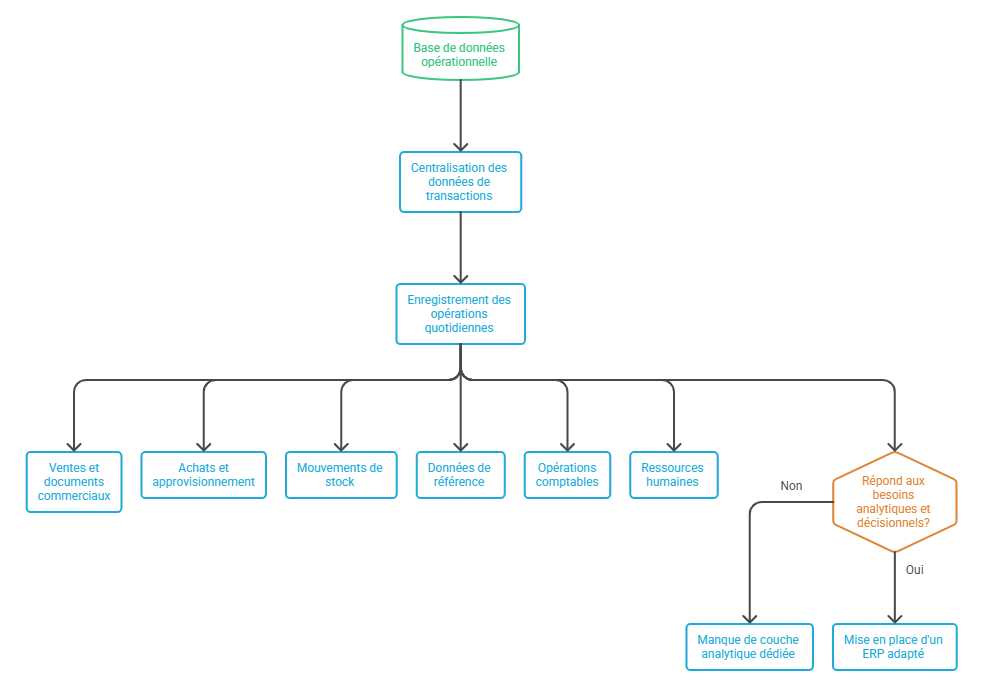
\includegraphics[width=\linewidth]{Figures/visual_selection_4.png}
\caption{Architecture du flux de données opérationnelles et évaluation des besoins décisionnels}
\label{fig:ch1:flux}
\end{figure}

\subsection{Données disponibles}
Au début du projet, bien que l’entreprise dispose d’un historique de données antérieur, une extraction de la base de données de BIOSPHERE a été déployée sur un environnement local, couvrant la période allant de 2019 à juillet 2025. Le choix de cet intervalle temporel s’avère particulièrement pertinent pour plusieurs raisons. D’une part, il inclut la période de la pandémie de COVID-19, qui a fortement impacté les dynamiques du marché. D’autre part, il englobe également la phase de reprise post-pandémique, caractérisée par des évolutions significatives des comportements d’achat et des flux d’approvisionnement. Cette continuité temporelle permet ainsi d’analyser les variations structurelles du marché et d’identifier des tendances clés, ce qui constitue un atout majeur pour les analyses exploratoires et les modèles prédictifs. Par ailleurs, l’utilisation de données récentes et cohérentes renforce la fiabilité et la pertinence des résultats obtenus.
Toutefois, ces données, initialement stockées dans une base opérationnelle, n’étaient pas directement exploitables à des fins décisionnelles. Elles ont nécessité des étapes préalables de nettoyage, de normalisation et de structuration afin de garantir leur qualité et leur conformité aux exigences de la Business Intelligence et de la Data Science.
Dans cette optique, le projet a débuté par un processus de valorisation des données brutes, reposant sur l’exploitation des tables suivantes :


\begin{table}[H]
\centering
\caption{Structure et contenu des données brutes}
\label{tab:ch1:donnees}
\begin{tabular}{|p{5cm}|p{5cm}|p{5.5cm}|}
\hline
\multicolumn{1}{|c|}{\textbf{Catégorie}} & 
\multicolumn{1}{c|}{\textbf{Tables}} & 
\multicolumn{1}{c|}{\textbf{Contenu principal}} \\
\hline
Articles & \texttt{biosphere.dbo.Art} & Codes, désignations, familles, infos produits \\ \hline
Documents commerciaux & \texttt{biosphere.dbo.Document} & En-têtes : ventes, achats, dates, tiers, montants \\ \hline
Lignes de documents & \texttt{biosphere.dbo.DocumentD} & Détails : produits, quantités, prix, montants \\ \hline
Nature des documents & \texttt{biosphere.dbo.DocumentN} & Types/natures des documents \\ \hline
Tiers & \texttt{biosphere.dbo.Tiers} & Clients et fournisseurs \\ \hline
Mouvements de stock & \texttt{biosphere.dbo.StoJou} & Entrées, sorties, retours, transferts, quantités \\ \hline
Historique global & Base opérationnelle BIOSPHERE & Données de 2019 à juillet 2025 \\ \hline
\end{tabular}
\end{table}

\subsection{Limites identifiées}
L'analyse de l'existant a mis en évidence plusieurs limites significatives qui justifient la mise en place d'un système décisionnel dédié.
\subsubsection{Limites liées à la gestion du stock}
La base de données opérationnelle de BIOSPHERE n'était pas appropriée pour l'analyse décisionnelle car elle était initialement conçue pour la gestion des transactions. C’est pour cela cette base de données présentait plusieurs limites notamment les données brutes qui n'avaient pas été préparées. Les informations étaient stockées sous leur forme opérationnelle, et par conséquent, il fallait effectuer un travail important pour extraire, protéger, nettoyer, normaliser et transformer ces données avant de pouvoir les utiliser dans un Data Warehouse.

\subsubsection{Limites liées au pilotage de la performance}
Le projet a également été confronté à des contraintes d’ordre infrastructurel et, plus particulièrement, à des problématiques liées à la qualité des données. En effet, la présence de valeurs manquantes et d’incohérences dans certaines configurations a affecté la complétude et la fiabilité des jeux de données exploités. Ces insuffisances ont eu un impact direct sur la performance et la robustesse de certains modèles analytiques et prédictifs, en introduisant des biais potentiels et en limitant la précision des résultats.
Afin de pallier ces limitations, des techniques de prétraitement des données ont été envisagées, notamment des stratégies d’imputation des valeurs manquantes, de détection et de correction des anomalies, ainsi que des procédures de validation visant à améliorer la qualité globale de l’information et à renforcer la fiabilité des analyses produites.

\subsection{Analyse SWOT}
Nous avons réalisé une analyse SWOT pour identifier les facteurs importants qui influencent BIOSPHERE. Cette analyse a mis en évidence les points forts de l'entreprise, tels que l'expertise métier, la présence sur plusieurs sites et l'offre complète de BIOSPHERE. Cependant, elle a également révélé des faiblesses, notamment l'absence d'un système décisionnel intégré et l'utilisation limitée des données historiques. 
L'analyse a également montré que BIOSPHERE peut profiter de la valorisation des données par la Business Intelligence et la Data Science pour améliorer la gestion de la performance et prévenir les risques de rupture de stock.
\begin{table}[H]
\centering
\caption{Analyse SWOT du projet BIOSPHERE}
\label{tab:ch1:swot}
\begin{tabular}{|p{6.5cm}|p{6.5cm}|}
\hline
\multicolumn{1}{|c|}{\textbf{Forces}} & 
\multicolumn{1}{c|}{\textbf{Faiblesses}} \\ 
\hline
\begin{itemize}
    \item Présence multisite (Tunis et Sfax)
    \item Offre complète : distribution, installation, maintenance, SAV
    \item Relations avec établissements de santé, laboratoires, professionnels
    \item Expertise médicale/biomédicale/scientifique
    \item Historique de données opérationnelles exploitable
\end{itemize} & 
\begin{itemize}
    \item Absence d'un système décisionnel intégré
    \item Exploitation limitée des données historiques
    \item Pilotage dépendant d'analyses manuelles/dispersées
    \item Manque de visibilité prévisionnelle sur les stocks et ruptures
\end{itemize} \\ \hline
\multicolumn{1}{|c|}{\textbf{Opportunités}} & 
\multicolumn{1}{c|}{\textbf{Menaces}} \\ 
\hline
\begin{itemize}
    \item Transformation digitale du secteur santé
    \item Valorisation des données via BI et Data Science
    \item Amélioration du suivi ventes/achats/stock via dashboards
    \item Optimisation des décisions d'achat et réapprovisionnement
\end{itemize} & 
\begin{itemize}
    \item Risques de rupture de stock impactant la satisfaction client
    \item Fluctuations des devises et coûts d'importation
    \item Évolution rapide des technologies médicales
    \item Contraintes réglementaires strictes du secteur médical
\end{itemize} \\ \hline
\end{tabular}
\end{table}
L’analyse SWOT de l’entreprise BIOSPHERE met en évidence un contexte globalement favorable à la mise en place d’une solution décisionnelle avancée. L’entreprise dispose de plusieurs atouts majeurs, notamment une présence multisite, une offre de services complète et une expertise solide dans le secteur médical et biomédical. Surtout, elle bénéficie d’un historique de données opérationnelles riche, constituant un levier essentiel pour l’exploitation analytique et prédictive.
Toutefois, cette analyse révèle également des faiblesses significatives, principalement liées à l’absence d’un système décisionnel intégré et à une exploitation limitée des données existantes. Le pilotage de la performance repose encore sur des approches manuelles et fragmentées, entraînant un manque de visibilité sur des indicateurs critiques tels que les niveaux de stock et les risques de rupture. De plus, la qualité des données constitue une contrainte importante, avec la présence d’incohérences et de valeurs manquantes.
En contrepartie, l’environnement externe offre de réelles opportunités, notamment à travers la transformation digitale du secteur de la santé et le développement des approches de Business Intelligence et de Data Science. Ces évolutions permettent d’envisager une meilleure valorisation des données, une amélioration du suivi opérationnel et l’intégration de modèles prédictifs pour optimiser la prise de décision.
Néanmoins, ces opportunités doivent être considérées à la lumière de certaines menaces, telles que les risques de rupture de stock, la volatilité des coûts d’importation, l’évolution rapide des technologies médicales ainsi que les contraintes réglementaires strictes du secteur. Dans ce contexte, la mise en place d’une solution BI et IA apparaît comme une réponse stratégique visant à renforcer la performance, la réactivité et la capacité prédictive de l’entreprise.

\section{Section 4 : Problématique et objectifs}
\subsection{Problématique}
Dans un contexte où les données opérationnelles sont disponibles mais insuffisamment exploitées, la question centrale est : \textit{Comment exploiter les données historiques de BIOSPHERE à travers une architecture décisionnelle intégrant Business Intelligence, Data Engineering et Machine Learning afin d’améliorer l’analyse des performances et d’anticiper les risques de rupture de stock ?}

Cette problématique principale se diversifie en deux sous-problématiques distinctes qui correspondent aux deux grandes composantes principales pour le projet et complémentaires :
\begin{enumerate}
    \item Comment fournir aux décideurs une vision claire et exploitable des ventes, achats et stock pour suivre la performance, détecter les anomalies et faciliter la prise de décision selon le rôle de chaque utilisateur ?
    \item Comment anticiper les risques liés au stock, notamment les ruptures, afin d’améliorer les décisions de réapprovisionnement et prioriser les actions ?
\end{enumerate}

\subsection{Objectifs}
L’objectif principal de ce projet est de concevoir et de mettre en place une solution décisionnelle intégrée pour l’entreprise BIOSPHERE, visant à améliorer la qualité de la prise de décision. Cette solution repose sur une architecture complète combinant la gestion des données, l’analyse métier, la modélisation prédictive et la restitution décisionnelle.
Elle se structure autour de quatre composantes majeures :\\
    • Une couche de gestion et de préparation des données (Data Engineering)\\
    • Une couche d’analyse et de restitution métier (Business Intelligence)\\
    • Une composante de modélisation et de prédiction (Data Science)\\
    • Une application décisionnelle centralisée destinée aux utilisateurs finaux.\\

Dans ce cadre, les objectifs spécifiques du projet s’articulent autour de cinq axes complémentaires :
\begin{enumerate}
    \item \textbf{Data Engineering :} Automatiser les processus de collecte, de nettoyage et de transformation des données à travers la mise en place d’un pipeline ETL robuste, fiable et reproductible.
    \item \textbf{Data Warehouse :} Concevoir et implémenter un entrepôt de données structuré regroupant les informations relatives aux ventes, aux achats et aux stocks, afin de faciliter l’analyse multidimensionnelle.
    \item \textbf{Business Intelligence :} Développer des tableaux de bord interactifs sous Power BI, sécurisés par un mécanisme de Row-Level Security (RLS), permettant le pilotage de la performance globale et le suivi des indicateurs de stock.
    \item \textbf{Data Science :} Mettre en œuvre des modèles prédictifs permettant d’anticiper les risques de rupture de stock et de prévoir les besoins sur un horizon de trois mois, à partir des données historiques.
    \item \textbf{Application décisionnelle :} Développer une interface unique et sécurisée, regroupant les analyses, les indicateurs clés et les alertes critiques, afin de faciliter l’accès à l’information et d’améliorer la réactivité décisionnelle.
\end{enumerate}
Ainsi, ce projet vise à transformer les données brutes de l’entreprise en un véritable levier stratégique, en combinant ingénierie des données, analyse descriptive et intelligence prédictive.
\begin{figure}[H]
\centering
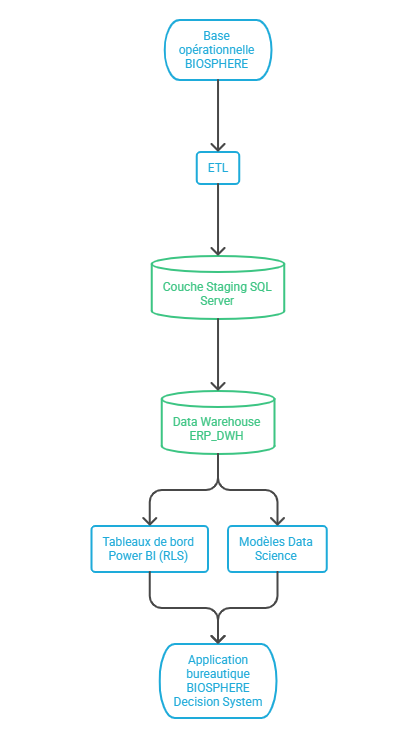
\includegraphics[width=0.8\linewidth]{Figures/visual_selection_5.png}
\caption{Chaîne décisionnelle globale du projet}
\label{fig:ch1:chaine}
\end{figure}

\section{Section 5 : Cadre théorique} 
Cette section présente de manière synthétique les fondements théoriques sur lesquels repose le projet BIOSPHERE BI & IA. Elle couvre les concepts essentiels de la Business Intelligence, du Machine Learning, ainsi que les choix techniques adoptés et leur justification. L'objectif est de fournir les clés de lecture nécessaires à la compréhension des réalisations décrites dans les chapitres suivants.
\subsection{Business Intelligence}
\subsubsection{Définition et rôle}
La Business Intelligence (BI) désigne l'ensemble des processus, technologies et outils qui permettent de collecter, d'intégrer, d'analyser et de présenter les données d'une organisation sous une forme exploitable par les consommateurs. \\
Selon Gartner, cité \cite{turban2011} dans les travaux de Turban et al., la Business Intelligence est définie comme « Business intelligence is an umbrella term that includes the applications, infrastructure and tools, and best practices that enable access to and analysis of information to improve and optimize decisions and performance » \\
Traduction : « un terme générique qui désigne les applications, les infrastructures, les outils et les meilleures pratiques permettant l’accès et l’analyse d’informations afin d’améliorer et d’optimiser les décisions et les performances » \cite{turban2011}\\
Dans le contexte d'une entreprise comme BIOSPHERE, la BI joue un rôle structurant : elle transforme les données transactionnelles brutes en des données enregistrées au quotidien dans un système opérationnel sous forme des indicateurs synthétiques, des tendances et des alertes exploitables par les responsables commerciaux et logistiques. Elle répond ainsi à des questions du type : quelles sont les ventes réalisées sur le dernier trimestre ? Quel est le niveau de stock disponible par site ? Quels produits affichent une marge insuffisante ?\

Le cycle de la BI comprend quatre étapes fondamentales : 
\begin{enumerate}
\item La collecte et l’intégration des données (ETL) 
\item Le stockage dans un entrepôt analytique (Data Warehouse)
\item L’analyse multidimensionnelle 
\item La restitution sous forme de tableaux de bord interactifs.
\end{enumerate}
\begin{figure}[H]
\centering

\includegraphics[width=0.8\linewidth]{Figures/visual_selection_6.png}
\caption{Processus Décisionnel de BIOSPHERE}
\label{fig:ch1:processus_bi}
\end{figure}
En résumé, la Business Intelligence, dans ce projet, est la première étape pour rendre les données utiles. Elle prend les données opérationnelles et les transforme en tableaux de bord faciles à comprendre. 

\subsubsection{Les outils de Business Intelligence}
Les outils de Business Intelligence sont véritablement utiles pour collecter les données, les analyser, les visualiser et les partager. Cela aide beaucoup à prendre des décisions éclairées et efficaces. 
Ces outils prennent les données des systèmes opérationnels ou des Data Warehouse et les transforment en indicateurs, en rapports et en tableaux de bord interactifs et dynamiques que l'on peut utiliser aisément. 
Il existe plusieurs solutions populaires, comme Power BI, Tableau, Qlik Sense et Looker, qui sont utilisées par de nombreuses entreprises.

\textbf{ a) Microsoft Power BI}\\
Définition :

Power BI est une plateforme de Business Intelligence développée par Microsoft. Elle permet de connecter différentes sources de données, de les transformer, de créer des modèles analytiques et de concevoir des tableaux de bord interactifs.

\begin{figure}[H]
\centering

\includegraphics[width=0.3\textwidth]{Figures/Microsoft-Power-BI-Logo.png}
\caption{Logo Microsoft Power BI}
\label{fig:powerbi_logo}
\end{figure}

Power BI offre plusieurs fonctionnalités :

\begin{itemize}
    \item Connexion à de multiples sources de données ;
    \item Transformation et préparation des données avec Power Query ;
    \item Modélisation des données avec DAX ;
    \item Création de tableaux de bord interactifs ;
    \item Publication et partage des rapports.
\end{itemize}

Limites :

\begin{itemize}
    \item Certaines fonctionnalités avancées nécessitent une licence payante ;
    \item Courbe d'apprentissage pour les expressions DAX ;
    \item Limitations de performance sur de très grands volumes de données.
\end{itemize}

\textbf{ b) Tableau}\\
Définition :

Tableau est une solution de Business Intelligence et d’analyse visuelle développée par Salesforce. Elle permet de connecter les données, puis de les explorer et de produire des visualisations interactives. Tableau se concentre particulièrement sur l’analyse visuelle et l’exploration intuitive des données.

\begin{figure}[H]
\centering

\includegraphics[width=0.3\textwidth]{Figures/Tableau-Logo.png}
\caption{logo du logiciel tableau}
\label{fig:tableau_logo}
\end{figure}

Limites :

Tableau peut être coûteux pour certaines entreprises d’une part, surtout lorsque plusieurs utilisateurs doivent accéder aux rapports ou collaborer sur une plateforme partagée. D’autre part, la préparation avancée des données peut nécessiter des outils complémentaires. De plus, même si l’interface est immédiate pour la visualisation, la construction de modèles analytiques complexes peut demander une expertise technique.

\textbf{c) Qlik Sense}\\
Définition :

Qlik Sense est une plateforme de Business Intelligence et d'analyse de données très utile développée par Qlik. Elle nous permet de créer des tableaux de bord interactifs, d'explorer les données et d'obtenir des analyses assistées par l'intelligence artificielle. 

\begin{figure}[H]
\centering

\includegraphics[width=0.3\textwidth]{Figures/Qlik_Logo.svg.png}
\caption{logo du logiciel Qlik Sense}
\label{fig:Qlik_SENSE_logo}
\end{figure}

Limites :

Qlik Sense peut nécessiter un temps d’apprentissage, exceptionnellement pour comprendre son modèle associatif et développer des applications analytiques avancées. Sa mise en place peut être complexe dans les environnements où les sources de données sont nombreuses ou bien évidements mal structurés.

\textbf{d) Looker}\\
Définition :

Un Data Warehouse, ou entrepôt de données, est une base de données analytique centralisée destinée à l’aide à la décision. Contrairement à une base opérationnelle, qui sert principalement à gérer les transactions quotidiennes, le Data Warehouse est conçu pour l’analyse, le suivi historique et la production d’indicateurs. 

\begin{figure}[H]
\centering

\includegraphics[width=0.3\textwidth]{Figures/Looker.svg.png}
\caption{logo du logiciel Qlik Sense}
\label{fig:Qlik_SENSE_logo}
\end{figure}

Limites :

Looker peut-être moins accessible pour des utilisateurs débutants, parce qu’il repose sur une logique de modélisation spécifique par exemple avec Look ML. Sa mise en œuvre demande donc des compétences techniques, en particulier pour pouvoir construire et maintenir la couche sémantique. Il est fortement orienté vers les environnements cloud, ce qui peut constituer une contrainte pour les entreprises qui souhaitent une solution totalement locale.

\subsection{Data Warehouse : concept et architecture}
Un Data Warehouse, ou entrepôt de données, est une base de données analytique centralisée destinée à l’aide à la décision. Contrairement à une base opérationnelle, qui sert principalement à gérer les transactions quotidiennes, le Data Warehouse est conçu pour l’analyse, le suivi historique et la production d’indicateurs.\\
Selon George \cite{george2024}: « Un Data Warehouse est un système centralisé qui consolide des données historiques et courantes provenant de sources hétérogènes, structuré selon un modèle analytique optimisé pour l'interrogation, l'analyse décisionnelle et la génération d'insights actionnables. Il se caractérise par quatre propriétés fondamentales : orientation métier (subject-oriented), intégration des sources, non-volatilité des données chargées, et variabilité temporelle permettant l'analyse historique » \\
Sur le plan architectural, un Data Warehouse repose généralement sur trois couches principales :\\
•	La couche de staging, qui reçoit, nettoie, prépare les données issues des sources opérationnelles et protège contre le crash.\\
•	La couche de stockage analytique, qui organise les données dans un modèle décisionnel.\\
•	La couche de restitution, qui permet l’exploitation des données à travers des rapports et tableaux de bord, comme Power BI dans ce projet.\\
Donc, le Data Warehouse constitue le cœur du système décisionnel.


\subsubsection{Modélisation dimensionnelle : Star, Snowflake et Galaxy}
La modélisation dimensionnelle est une méthode très utilisée pour concevoir un Data Warehouse. Elle se base sur deux types de tables : les tables de faits et les tables de dimensions. 
Les tables de faits contiennent les mesures quantitatives liées à l’activité de l’entreprise, comme les montants ou les quantités. En revanche, Les tables de dimensions contiennent les informations descriptives qui permettent d’analyser ces mesures de différentes manières, par exemple en fonction du produit, du client, du fournisseur, de la date ou du site. Cette structure rend l’analyse des données et la production d’indicateurs décisionnels beaucoup plus faciles. 

Dans la modélisation décisionnelle d’un Data Warehouse, on distingue principalement trois principaux schémas de modélisation :

\begin{itemize}
    \item \textbf{Schéma en étoile} 
    \begin{figure}[H]
\centering
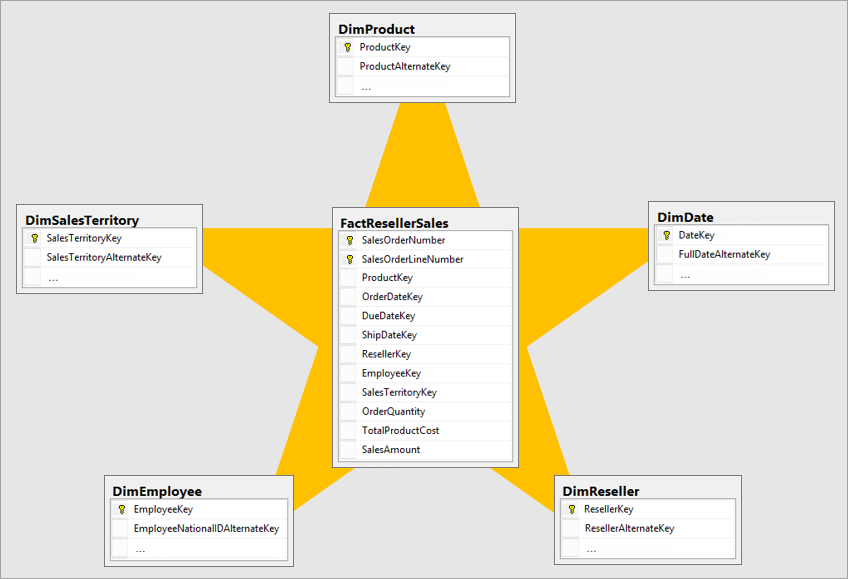
\includegraphics[width=0.6\linewidth]{Figures/star_schema.png}
\caption{Schéma en étoile}
\label{fig:ch1:Star Schema}
\end{figure}
    Chaque table de faits est directement reliée à ses dimensions. Simple et performant, il est adapté aux analyses portant sur un seul processus métier
    \item \textbf{Schéma en flocon de neige} 
    \begin{figure}[H]
\centering
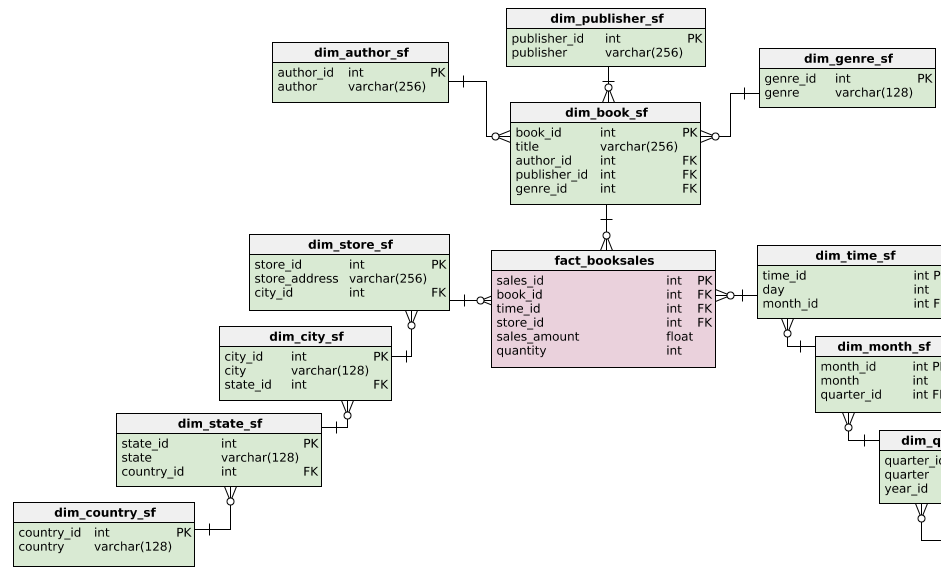
\includegraphics[width=0.8\linewidth]{Figures/book-snowflake-copy.png}
\caption{Schéma en flocon de neige}
\label{fig:ch1:snowflake}
\end{figure}
    Les dimensions sont normalisées en sous-dimensions. Plus économe en espace de stockage, mais plus complexe à interroger.
    \item \textbf{Schéma en Galaxy } 
    \begin{figure}[H]
\centering
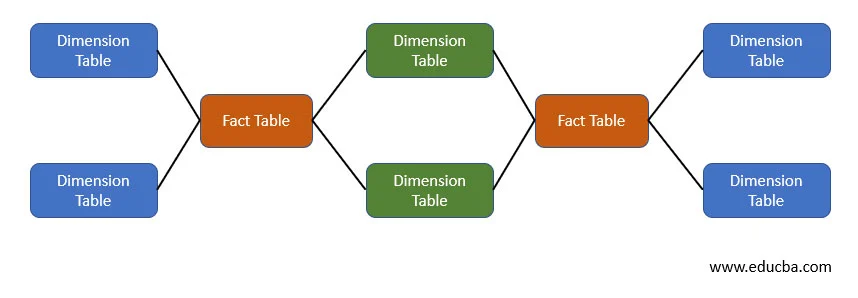
\includegraphics[width=0.9\linewidth]{Figures/Fact-Constellation-Schema1.png}
\caption{Schéma en Galaxy}
\label{fig:ch1:star}
\end{figure}
    Un schéma en galaxie est un modèle de Data Warehouse composé de plusieurs tables de faits reliées à des dimensions communes. Il est utilisé lorsqu’un projet analyse plusieurs processus métier en même temps, comme les ventes, les achats et le stock.
\end{itemize}
D’autres approches existent, comme le Data Vault ou le modèle relationnel normalisé, mais elles sont généralement utilisées dans des contextes plus spécifiques ou plus complexes.


\subsection{Processus ETL}
\subsubsection{Définition du processus ETL}
Le processus ETL est un processus crucial qui aide à transférer les données des systèmes opérationnels vers un endroit où nous pouvons les analyser, transformer et même protéger, comme un Data Warehouse. Ce processus permet de préparer, de rendre fiables et d'organiser les données pour qu'elles soient cohérentes et prêtes à être utilisées pour prendre des décisions ou pour l’application du IA.
Dans un système qui aide à prendre des décisions, l'ETL est vraiment important. Il assure que les données que nous utilisons pour les rapports, les tableaux de bord et les indicateurs viennent de sources sûres et sont organisées d’une manière efficace. Cela permet de relier les données brutes de l'entreprise aux outils d'analyse.


\subsubsection{Les trois étapes du ETL}
\begin{enumerate}
    \item \textbf{Extract (Extraction):} C’est l’action de récupération les données depuis les bases sources.
    \item \textbf{Transform (Transformation) :} Correspond aux traitements du nettoyage, standardisation, enrichissement et restructuration des données. Cette étape comprend notamment la normalisation des formats de dates, la conversion des types numériques, le traitement des valeurs incohérentes (vide ou fausse) et la génération des clés techniques.
    \item \textbf{Load (Chargement):} c’est l’action Insertion des données transformées dans le Data Warehouse. Le chargement peut être complet (full load) ou incrémental (incremental load), selon la logique de mise à jour adapté.
\end{enumerate}

\subsubsection{Les outils ETL}
Un outil ETL est une solution logicielle qui permet de concevoir, automatiser, exécuter et surveiller des workflows d’intégration de données. Il assure le passage des données depuis les systèmes sources vers un environnement analytique, comme un Data Warehouse, en garantissant leur préparation, leur cohérence et leur fiabilité pour l’analyse décisionnelle.
Parmi les outils ETL les plus connus, on peut citer :

\begin{itemize}
    \item \textbf{Talend } 
    \begin{figure}[H]
\centering

\includegraphics[width=0.3\linewidth]{Figures/Logo-talend.jpg}
\caption{logo du logiciel Talend}
\label{fig:ch1:logiciel Talend}
\end{figure}
    Est un outil d’intégration de données permettant de créer des flux ETL visuels. Il est utilisé pour connecter plusieurs sources, transformer les données et alimenter des Data Warehouses.  
    \item \textbf{Microsoft SQL Server Integration Services (SSIS) } 
    \begin{figure}[H]
\centering

\includegraphics[width=0.3\linewidth]{Figures/ssis-logo.png.jpg}
\caption{logo du logiciel Microsoft SQL Server Integration Services}
\label{fig:ch1:logo du logiciel Microsoft SQL Server Integration Services}
\end{figure}
    Est un outil ETL intégré à l’écosystème Microsoft, souvent utilisé avec SQL Server pour automatiser les flux de données.  
    \item \textbf{Apache Airflow } 
    \begin{figure}[H]
\centering

\includegraphics[width=0.3\linewidth]{Figures/AirflowLogo.png}
\caption{logo logiciel Apache Airflow}
\label{fig:ch1:logiciel Apache Airflow}
\end{figure}
    Est un outil d’orchestration de workflows permettant de planifier et surveiller des pipelines de données. 
    \item \textbf{n8n} 
        \begin{figure}[H]
\centering

\includegraphics[width=0.3\linewidth]{Figures/vertical-align.png}
\caption{logo logiciel n8n}
\label{fig:ch1:logo logiciel n8n}
    \end{figure}
    Est un outil d’automatisation de workflows qui permet de connecter plusieurs services et bases de données. 
\end{itemize}

\subsection{Machine Learning}
\subsubsection{Définition}
Le Machine Learning ou l’apprentissage automatique est une branche de l'intelligence artificielle qui regroupe l'ensemble des méthodes permettant à un système informatique d'apprendre à partir de données, sans être explicitement programmé pour chaque tâche. 
Selon Zhang : « Le Machine Learning désigne un ensemble de méthodes algorithmiques permettant aux systèmes d’extraire automatiquement des connaissances à partir de données, d’ajuster leurs paramètres par optimisation itérative et d’améliorer progressivement leurs performances prédictives ou décisionnelles sur des tâches spécifiques, sans programmation explicite des règles » (Zhang, 2024)
De manière générale, le Machine Learning permet de :
-	Automatiser certaines tâches complexes.
-	Prédire des résultats futurs à partir de données historiques.
-	Classer des observations en différentes catégories. 
-	Détecter des anomalies ou des comportements inhabituels. 
-	Améliorer la prise de décision à partir de données. 
-	Adapter les systèmes à de nouvelles situations grâce à l’apprentissage.
Mais malgré ses avantages, le Machine Learning présente plusieurs limites tel que ses performances dépendent fortement de la qualité des données utilisées c’est-à-dire que si les données sont incomplètes, bruitées, biaisées ou mal représentatives, les résultats du modèle peuvent être incorrects ou peu fiables.
Ainsi, le surapprentissage du modèle, ou overfitting qui se produit lorsqu’un modèle apprend trop précisément les données d’entraînement, au point de mal généraliser sur de nouvelles données.
Le Machine Learning peut aussi être difficile à interpréter, surtout lorsque les modèles utilisés sont complexes. Dans certains cas, il devient compliqué d’expliquer pourquoi le modèle a produit une prédiction particulière.
Enfin, les modèles de Machine Learning ne garantissent pas une prédiction parfaite. Ils fournissent des résultats probabilistes ou estimatifs, qui doivent être interprétés avec prudence. Ils nécessitent également une mise à jour régulière lorsque les données, les comportements ou le contexte évoluent.

\subsubsection{Types d'apprentissage}
On distingue classiquement trois grandes familles d'apprentissage automatique, selon la nature des données disponibles et l'objectif de modélisation :
\begin{itemize}
    \item \textbf{Supervisé :} Le modèle apprend à partir d'exemples étiquetés, où chaque observation est associée à une valeur cible connue. Cela est très utilisé dans la pratique, notamment pour les problèmes de classification et de régression. Nous utilisons ce type d'apprentissage dans ce projet pour les deux axes Data Science.
    \item \textbf{Non supervisé :} Le modèle identifie des structures cachées dans des données qui ne comportent pas d'étiquettes. Les algorithmes de regroupement, tels que K-Means et DBSCAN, ainsi que les algorithmes de réduction de dimension, comme l'analyse en composantes principales, en sont des exemples typiques.
\end{itemize}

\begin{figure}[H]
\centering
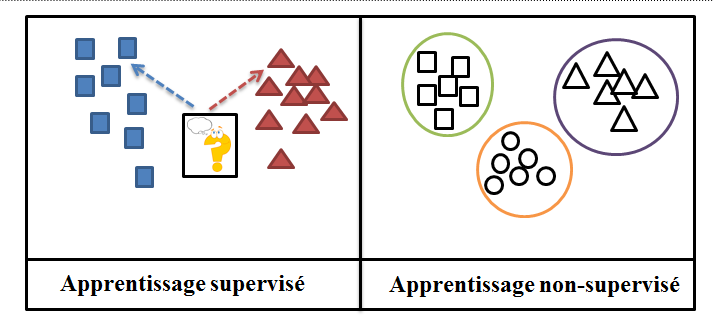
\includegraphics[width=0.7\linewidth]{Figures/apprentissage_supervise_vs_non_supervise.png}
\caption{L'apprentissage supervisé et non supervisé}
\label{fig:ch1:ml_types}
\end{figure}

\subsubsection{Classification et régression}
Dans le cadre de l'apprentissage supervisé, deux types de problèmes fondamentaux sont distingués selon la nature de la variable cible à prédire :
\begin{table}[H]
\centering
\caption{Comparaison entre classification et régression}
\label{tab:ch1:ml_comp}
\begin{tabular}{|p{3cm}|p{5cm}|p{5cm}|}

\hline
\multicolumn{1}{|c|}{\textbf{Critère}} & 
\multicolumn{1}{c|}{\textbf{Classification}} & 
\multicolumn{1}{c|}{\textbf{Régression}} \\ \hline
Variable cible & Catégorielle / discrète & Continue / numérique \\ \hline
Question posée & À quelle classe appartient cet exemple ? & Quelle valeur numérique prévoir ? \\ \hline
Métriques typiques & Accuracy, F1-score, ROC-AUC & MAE, RMSE, R² \\ \hline
Modèles courants & Random Forest, XGBoost & Régression linéaire, Random Forest \\ \hline
\end{tabular}
\end{table}

\subsection{Choix techniques du projet}
\subsubsection{Architecture décisionnelle retenue}
Le projet BIOSPHERE a une architecture décisionnelle bien organisée. Celle-ci est divisée en cinq niveaux différents. Cette organisation est faite pour respecter les règles de base de l'ingénierie des données. Les couches fonctionnelles sont clairement séparées, ce qui facilite la compréhension et la mise en œuvre du projet BIOSPHERE. Le projet BIOSPHERE comprend ces cinq niveaux successifs :
\begin{enumerate}
    \item \textbf{Couche source :} base opérationnelle SQL Server de BIOSPHERE, contenant les données transactionnelles brutes
    \item \textbf{Couche ETL :} pipeline orchestré par n8n dans Docker, assurant l'extraction, la transformation et le chargement incrémental des données
    \item \textbf{Couche staging :} base intermédiaire SQL Server, zone tampon de fiabilisation et de préparation des données
    \item \textbf{Couche analytique :} Data Warehouse ERP DWH en galaxy schéma, structurant les données de ventes, d'achats et de stock
    \item \textbf{Couche applicative :} tableaux de bord Power BI et application bureautique Python pour la restitution et l'aide à la décision
\end{enumerate}
Cette architecture garantit l'indépendance entre les couches, la traçabilité des transformations et la possibilité d'enrichir le système sans remettre en cause l'existant.
\subsubsection{Technologies mobilisées et justification}

Le tableau suivant présente les principales technologies retenues dans le cadre du projet, leur rôle dans l'architecture et la justification du choix effectué.

\begin{table}[H]
\centering
\caption{Technologies retenues dans le projet et justification}
\label{tab:ch1:tech}
\begin{tabular}{|p{3cm}|p{4cm}|p{7cm}|}
\hline
\multicolumn{1}{|c|}{\textbf{Technologie}} & 
\multicolumn{1}{c|}{\textbf{Rôle}} & 
\multicolumn{1}{c|}{\textbf{Justification}} \\ \hline
Docker Desktop & Conteneurisation & Isolation, reproductibilité et portabilité de l'environnement ETL \\ \hline
n8n & Orchestration ETL & Open source, léger, visuel, extensible, sans licence commerciale \\ \hline
SQL Server & Source, Staging, DWH & Cohérence avec l'existant, intégration facilitée, performances \\ \hline
Power BI & Visualisation BI & Intégration RLS native, connexion directe SQL, référence marché \\ \hline
Python & Data Science \& App & Écosystème ML (scikit-learn, pandas), développement d'app locale \\ \hline
CustomTkinter & Interface App & Bibliothèque moderne, fonctionnement local autonome sans cloud \\ \hline
scikit-learn & Modélisation ML & Implémentation robuste des algorithmes supervisés utilisés \\ \hline
\end{tabular}
\end{table}

\section{Conclusion}
Ce premier chapitre a permis de présenter le projet dans son contexte institutionnel et opérationnel dont la présentation de BIOSPHERE montre que l'entreprise dispose d'un patrimoine de données riche, varié et structuré, mais qu'elle n'a pas encore réussi à être bien utiliser pour prendre des décisions éclairées. Puis, l’analyse de l'existant a mis en lumière les défis à relever, résumés par une problématique centrale : comment transformer ces données brutes en leviers décisionnels et prédictifs ? Les cinq objectifs spécifiques définis répondent à cette question et tracent le périmètre du projet. Par la suite, une présentation de la théorie qui fondent les choix techniques et méthodologiques du projet pour justifier scientifiquement et techniquement chaque décision prise lors de la réalisation du projet. 

\newpage